\begin{frame}[fragile]
  \frametitle{Debugging Parallel Applications}
  \begin{itemize}
    \item It can be very difficult
    \item The typical ``printf'' strategy may be insufficient
    \item Using \texttt{gdb}
      \begin{itemize}
      \item Very easy with Charm++!
      \item Just run the application with the \texttt{++debug} command line
        parameter and a \texttt{gdb} window for each PE will open through X (and
        can be forwarded)
        \begin{itemize}
        \item Not very scalable
        \end{itemize}
      \end{itemize}
    \item We have developed a scalable tool for debugging Charm++ applications
      \begin{itemize}
      \item It's interactive
      \item Allows you to change message order to find bugs!
      \item ``What-if'' scenarios can be explored using provisional message
        delivery
      \item Memory can be tracked to find memory leaks
      \end{itemize}
  \end{itemize}
\end{frame}


\begin{frame}[fragile]
  \frametitle{Overview of CharmDebug}
  \begin{center}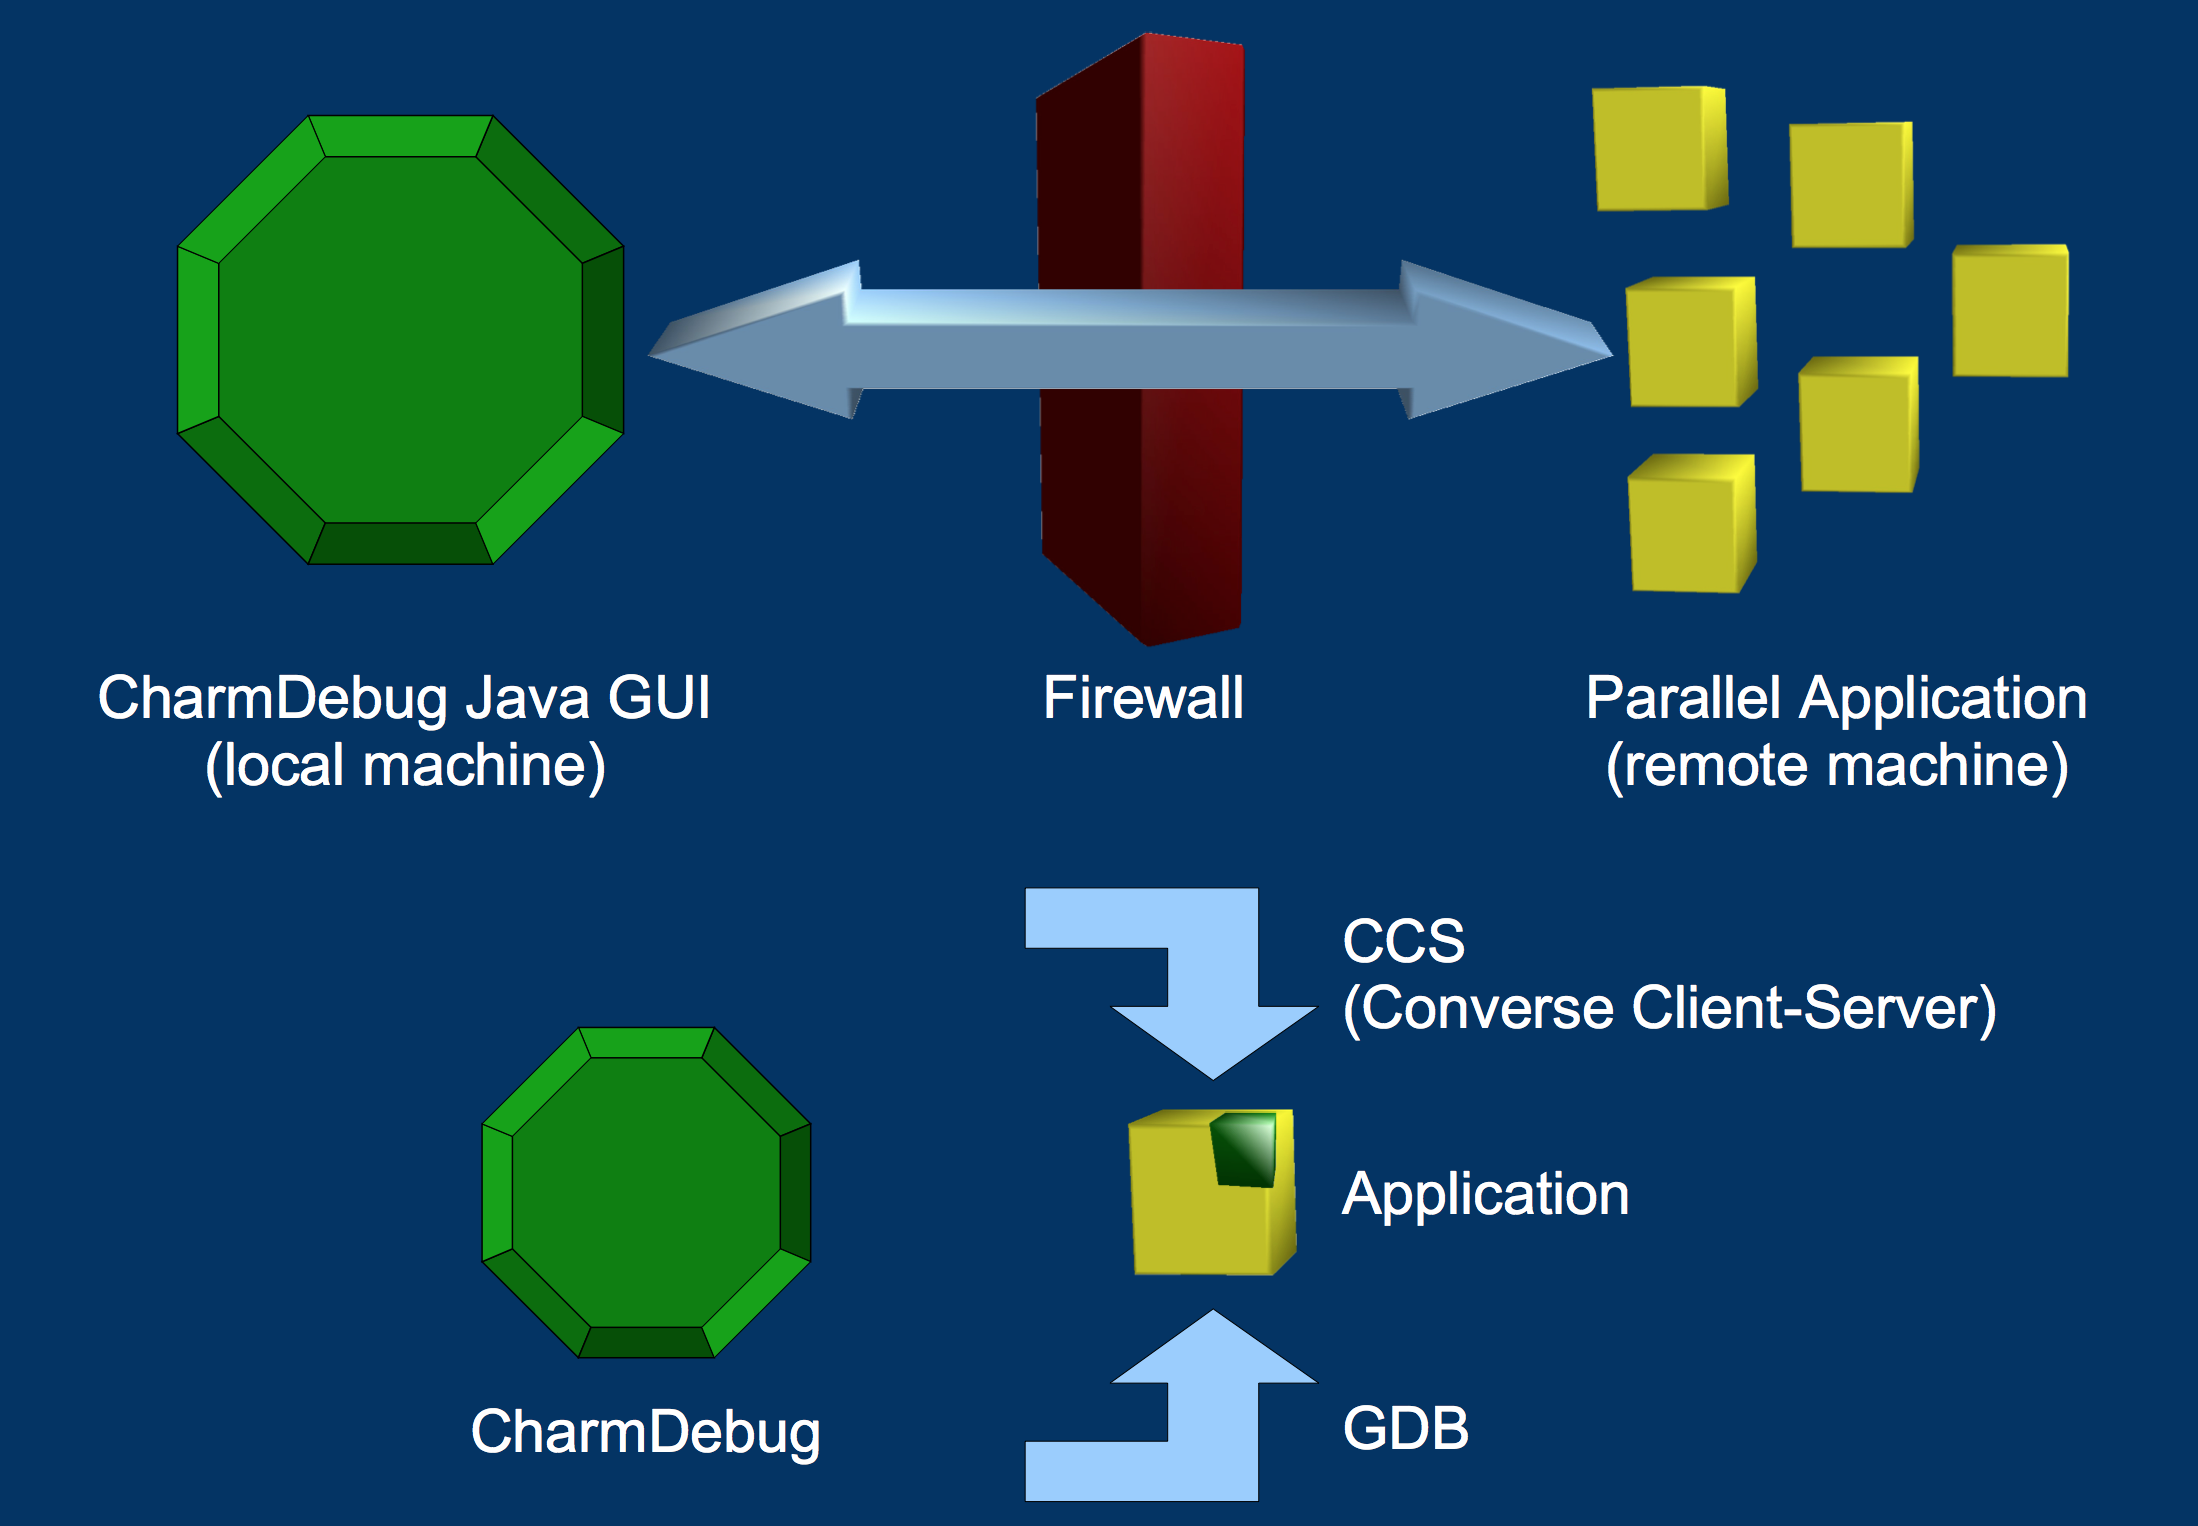
\includegraphics[width=0.9\textwidth]{figures/overviewDebug.png}\end{center}
\end{frame}

\begin{frame}[fragile]
  \frametitle{CharmDebug}
  \begin{center}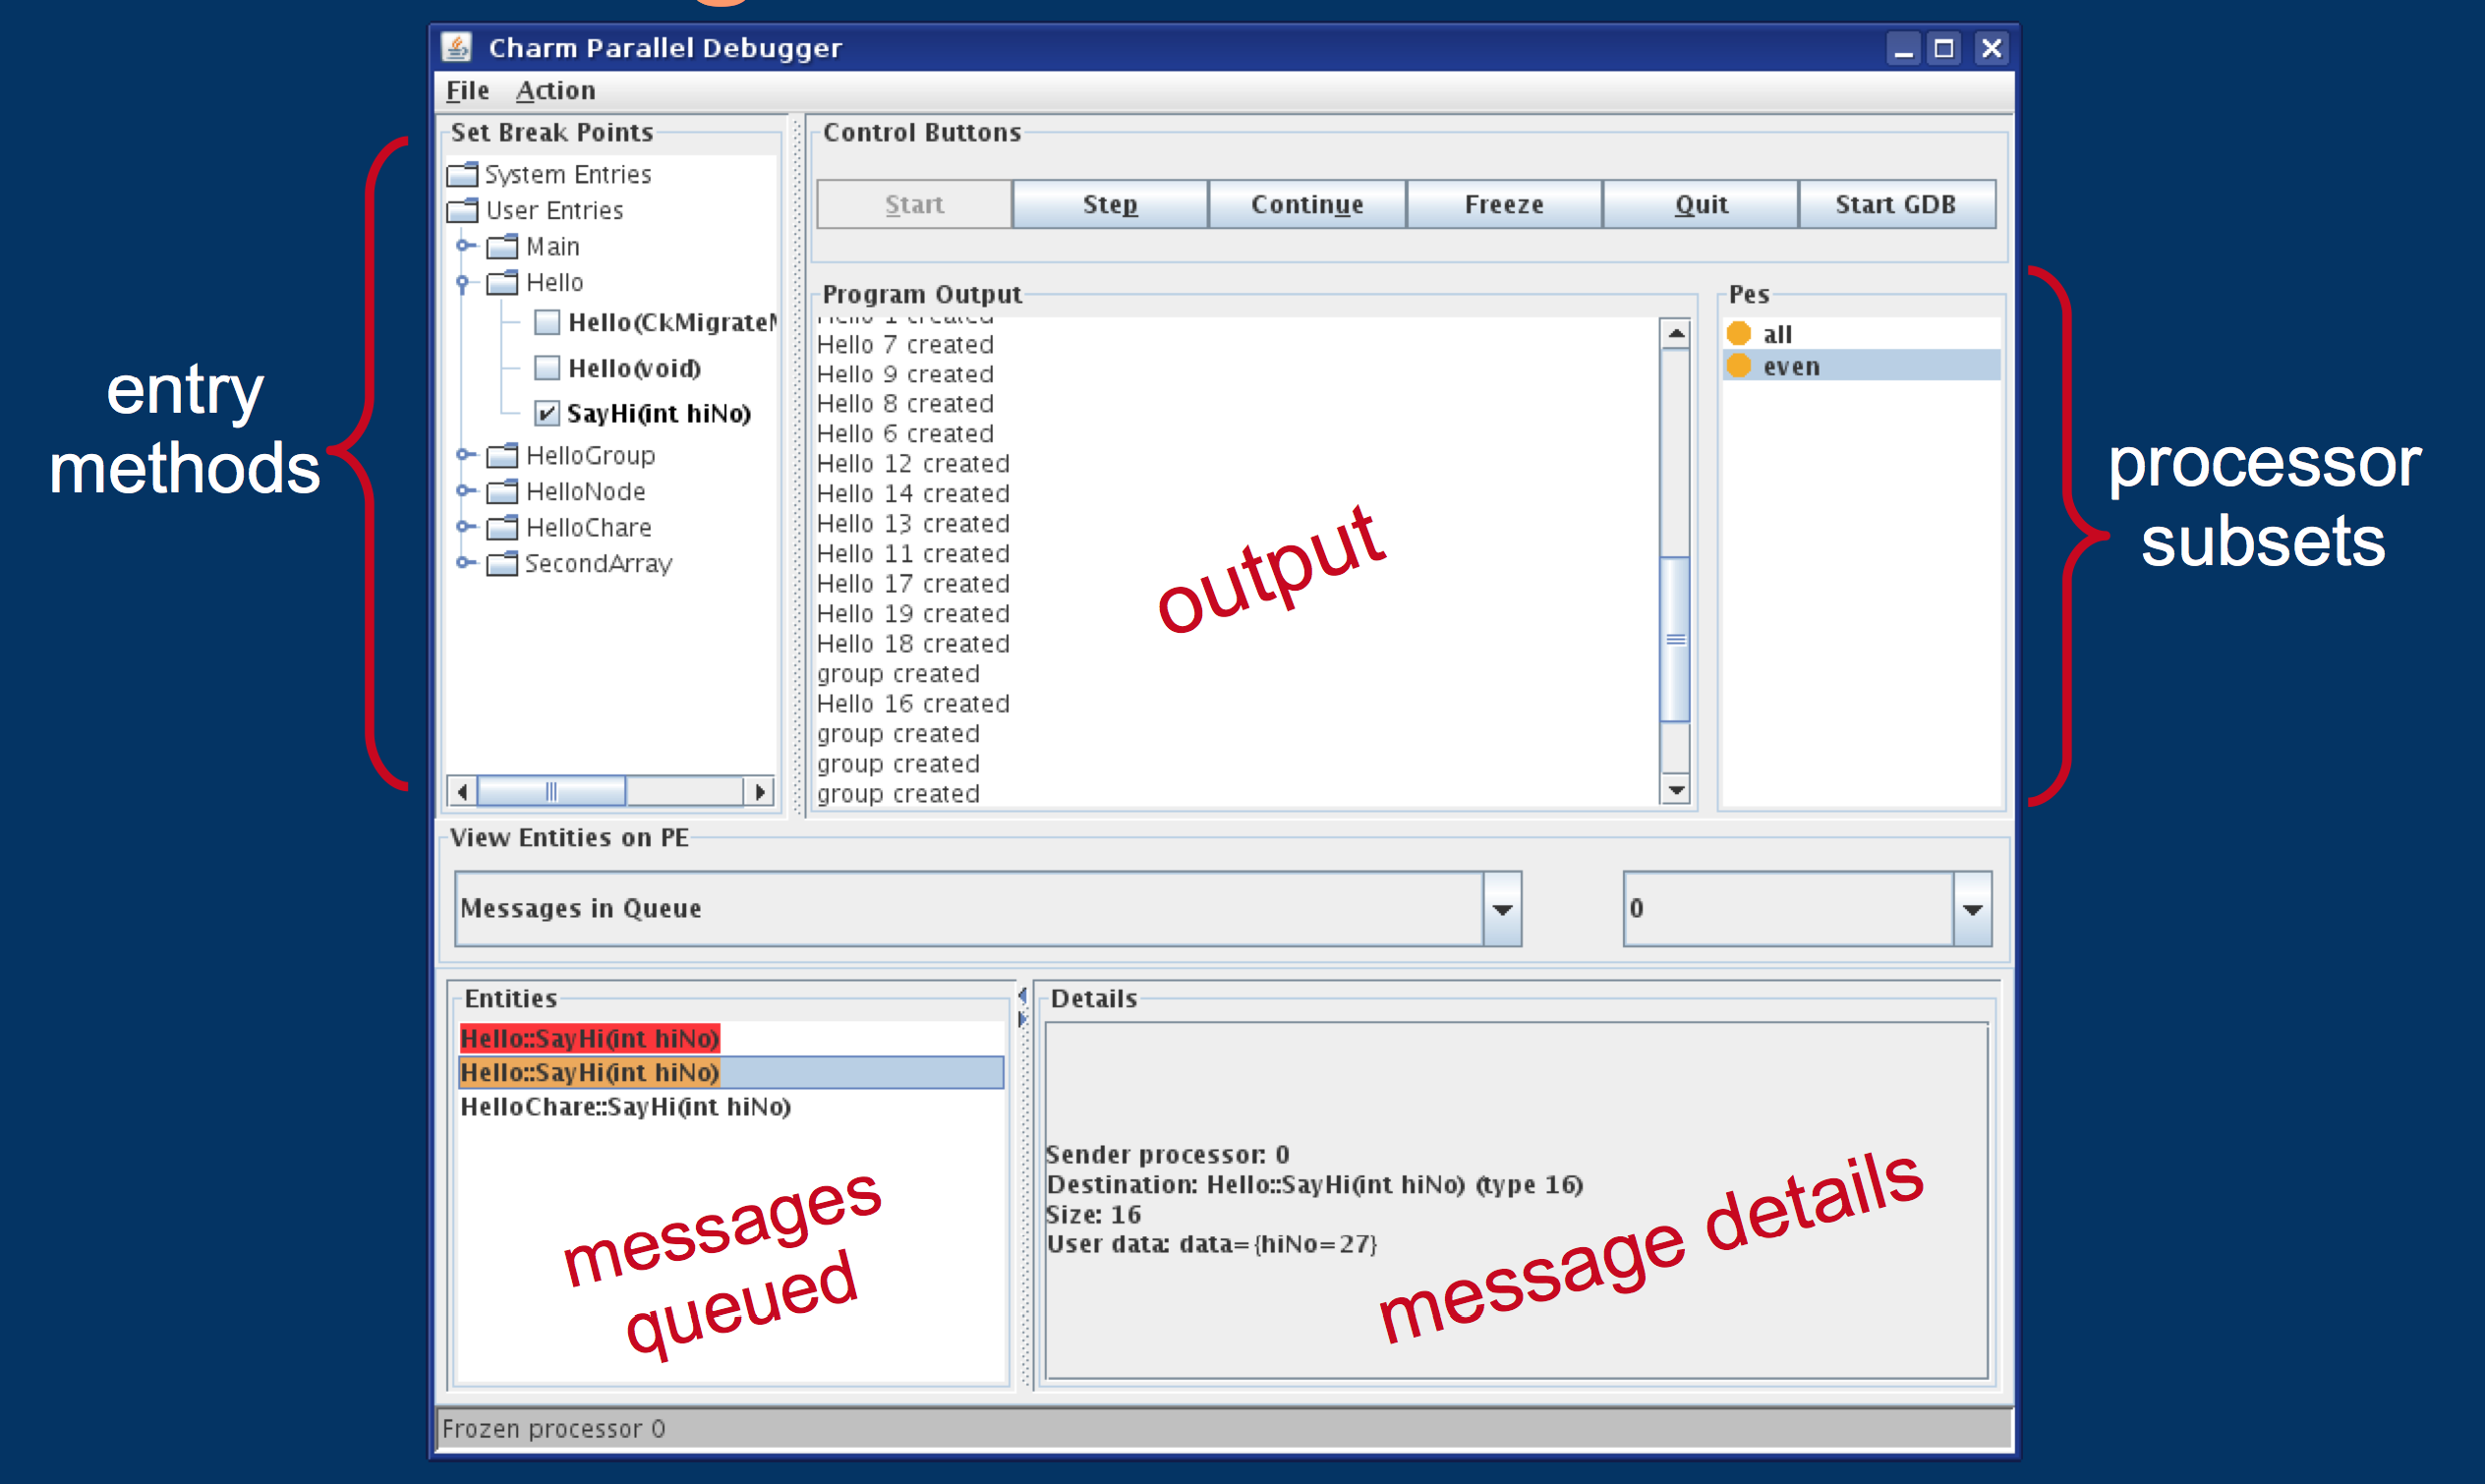
\includegraphics[width=0.9\textwidth]{figures/debugMainView.png}\end{center}
\end{frame}

\begin{frame}[fragile]
  \frametitle{Getting CharmDebug}
  \begin{itemize}
    \item It is part of Charm++
    \item For the basic feature set, nothing special needs to be done
    \item Precompiled for java 6
      \begin{itemize}
      \item Use \code{ant} to recompile
      \end{itemize}
    \item Help
      \begin{itemize}
      \item \verb|charm@cs.illinois.edu| (preferred)
      \item \verb|ppl@cs.illinois.edu|
      \end{itemize}
  \end{itemize}
\end{frame}

\begin{frame}[fragile]
  \frametitle{Compiling Your Applications}
  \begin{itemize}
    \item Charm++
      \begin{itemize}
      \item Use \texttt{-g}
      \item No \texttt{­-O3} or \texttt{--with-production}
      \end{itemize}
    \item Application
      \begin{itemize}
      \item Just compile with \texttt{-g}
      \item OR
      \item Compile with \texttt{-debug}
        \begin{itemize}
        \item Adds \texttt{­-g} \texttt{-­O0}, \texttt{--memory charmdebug}, Python
          modules
        \end{itemize}
      \end{itemize}
  \end{itemize}
\end{frame}

\begin{frame}[fragile]
  \frametitle{Launching in Debug Mode}
  \begin{itemize}
    \item Attach to running application in net- build
      \begin{itemize}
      \item Uses CCS to receive application output
      \end{itemize}
    \item Attach to running application in other builds
      \begin{itemize}
      \item Read the output file of the application
      \end{itemize}
    \item Start a new application in net- build
      \begin{itemize}
      \item Can use tunnels
      \end{itemize}
    \item Options available also in command line
      \begin{itemize}
      \item Use \verb|charmdebug ­help| to see them
      \end{itemize}
  \end{itemize}
\end{frame}
